\documentclass[twocolumn,apj,numberedappendix,appendixfloats]{openjournal}
% Available options:
% [twocolumn] - two-column mode
% [onecolumn] - (default) main text in one-column mode
% [apj]       - typeset in the style of ApJ.
% [apjl]      - (default) typeset in the style of ApJ Letters 
% [tighten]   - some adjustments to approximate grid typesetting
% [numberedappendix]   - number appendix sections as A, B, etc
% [appendixfloats]  - use separate numbering for floats within appendix
% [twocolappendix]  - make appendix in two-col mode in a two-col paper


%%%%% PACKAGES %%%%%
% Optional useful packages
\usepackage{newtxtext,newtxmath,amsmath}
\usepackage[T1]{fontenc}
\usepackage{graphicx}
\usepackage{enumitem}
\usepackage{xcolor}
\usepackage{hyperref}
\usepackage{gensymb}
\usepackage{CJK}
\usepackage{tabularx}
\usepackage{orcidlink}
\hypersetup{
    unicode, 
    colorlinks=true,
    linkcolor=linkcolor,
    citecolor=linkcolor,
    filecolor=linkcolor,
    urlcolor=linkcolor,
}
\definecolor{linkcolor}{rgb}{0.0,0.3,0.5}


% \usepackage{newtxtext,newtxmath,amsmath}
% \usepackage{xcolor}
% \usepackage{textgreek}
% \usepackage[utf8]{inputenc}
% \usepackage[english]{babel}
% \usepackage{hyperref}
% \hypersetup{
%     unicode, 
%     colorlinks=true,
%     linkcolor=linkcolor,
%     citecolor=linkcolor,
%     filecolor=linkcolor,
%     urlcolor=linkcolor,
% }
% \usepackage{color,colortbl}
% \definecolor{linkcolor}{rgb}{0.0,0.3,0.5}
% \usepackage{orcidlink}

%%%%% COMMANDS %%%%%
% Optional useful commands

% I use the following command to indicate comments with \SB{My comment here}.
% Before submission, you should comment this \newcommand out,
% to make sure you do not have any leftover comments!
\newcommand{\SB}[1]{{\textcolor{purple}{SB: #1}}}
\newcommand{\comment}[1]{\textcolor{lightgray}{#1}}

%%%%%%%%%%%%%%%%%%%%%%%%%%%%%%%%%%%%%%%%%%%%%%%%%
%%%%%%%%%%%%%%%%%%%%%%%%%%%%%%%%%%%%%%%%%%%%%%%%%
\begin{document}
\title{Interesting and descriptive title of your research}

\author{\vspace{-1.5cm}YOUR NAME HERE$^{1}$\orcidlink{0000-0000-0000-0000}}

% Adding another author would go like:
%\author{Sven Buder$^{1,2,*}$\orcidlink{0000-0002-4031-8553}}

\affiliation{$^{1}$Research School of Astronomy and Astrophysics, Australian National University, Canberra, ACT 2611, Australia}
% \affiliation{$^{2}$ARC Centre of Excellence for All Sky Astrophysics in 3 Dimensions (ASTRO 3D), Australia}


\thanks{E-mail: youremail@anu.edu.au}
%\thanks{$^*$Australian Research Council DECRA Fellow},

\begin{abstract}
The abstract should condense the main content of the paper to less than 1920 characters (with spaces) and make the reader want to actually read the paper. Summarize your work with at least one sentence for: context (bigger picture - to get people interested), aims (to tell people what you want to do), methods (to tell people how you do it), results (to give people important results, like numbers or rejected hypotheses), and conclusions (to explain the impact, that is, what that means for the bigger picture problem).
\end{abstract}

% Write your keywords here
\begin{keywords}
    {Choose up to 6 keywords from \href{https://academic.oup.com/DocumentLibrary/mnras/keywords.pdf}{here} and write them like: keyword1 -- keyword2.}
\end{keywords}

\maketitle

%%%%%%%%%%%%%%%%%%%%%%%%%%%%%%%%%%%%%%%%%%%%%%%%%
%%%%%%%%%%%%%%%%%%%%%%%%%%%%%%%%%%%%%%%%%%%%%%%%%
\section{Before you get started}

\subsection{How to do science and write papers}

\comment{When writing a scientific paper and doing research, always keep the scientific method in mind! You want your hypotheses be laid out clearly. Most importantly, you want to perform scientific research that is reproducible and statistically as well as logically sound! People may dispute the conclusions that you draw from your analyses, so always back up statements with logical and analytical arguments or at least with quantities and uncertainties. If you submit your research paper to a journal, an anonymous referee will be asked to review your study with the following questions in mind \citep{Bertout2004}:
\begin{enumerate}
    \item Why should this paper be published?
    \item Are the assumptions spelled out clearly?
    \item Are the methods fully described?
    \item Are the new results adequately emphasized?
    \item Are all the figures and tables necessary and properly laid out?
    \item \dots
    \item (different journals also may ask different questions)
\end{enumerate}}

\comment{The journals have a typical format of sections with introduction, data, methodology/analysis, results, discussion, conclusions. For ease, I have already created sections on clear pages that you can adjust (take out the clearpage command to save white space).}

\subsection{Coding and writing collaboratively}

\comment{Because you often do research with others (either your supervisors or a collaboration), it is vital that you are able to share your results, code, and manuscript. There are many ways to do that, including sending PDFs via emails.}

\comment{A common way is, however, to write code on your computer and then synchronize it with a server of an online service such as \url{https://github.com}. This is in fact where this template is stored at\footnote{\url{https://github.com/svenbuder/template_ojap}}. I would recommend to create a private repository for your research project to upload your code, figures, and manuscript.}

\comment{For writing, I use a hybrid of writing on my computer and the collaborative online service \url{https://www.overleaf.com/}. You can get free educational/professional versions of both GitHub and Overleaf with your ANU account and create private, that is, non-public repositories -- and even better: synchronize your GitHub repository with your Overleaf project (GitHub -> New Project -> Import from GitHub). Once you do that, you can invite collaborators to your project and make sure they always see your latest code and manuscript. Once you are ready to publicly share your code and manuscript, you simply just need to switch your repository type from \textit{private} to \textit{public}. This is how people can for example access the code and figures of my latest paper \citep{Buder2024} at \href{https://github.com/svenbuder/Accretion_Clues_ObsSim}{this} GitHub repository.}

\clearpage
\section{Introduction}
\label{sec:introduction}

\comment{The introduction is a condensed version of your literature review. You should start with the bigger picture and tell a story that naturally leads to your hypotheses and guides the structure of your paper.}

\comment{Remember to start from the big picture and the big questions that we want to answer, and use the introduction to reach the specific questions that you want to answer (and later link back) -- like an hourglass. The Decadal Plan of Australian Astronomy 2016--2025 \textit{Australia in the era of global astronomy}\footnote{You can find it \href{https://www.science.org.au/supporting-science/science-sector-analysis/reports-and-publications/decadal-plan-australian-astronomy-2016-25}{here}.} for example identifies 6 major questions that Australian astronomers want to tackle in the next decade: 
\begin{enumerate}
    \item How did the first stars and galaxies transform the Universe?
    \item What is the nature of dark matter and dark energy?
    \item How do galaxies form and evolve across cosmic time?
    \item How do stars and planets form?
    \item How are elements produced by stars and recycled through galaxies?
    \item What is the nature of matter and gravity at extreme densities?
\end{enumerate}}

\subsection{Scientific motivation}

\comment{\textit{The introduction should state clearly why the study was started and place the research in a broad context e.g. by referring to previous work of relevance. The introduction should not contain the conclusions.}\footnote{Taken from \href{https://www.aanda.org/doc_journal/instructions/aadoc.pdf}{these instructions}.}.}

\comment{It can be difficult to start, so here are a few pointers. Start by reading review papers in the specific area of your research. There is typically one ground-breaking or influential paper that is motivating your work (e.g. some new data or some new theoretical prediction). Read that paper too.}

\comment{The best way to find papers is via \href{https://ui.adsabs.harvard.edu}{the ADS service}. This service provides the link to the papers, publishers, and the \texttt{bibtex} information (on left side under \textit{Export Citation}). Add this \texttt{bibtex} information to a \LaTeX bibliography (\texttt{*.bib}) file in the same directory as your manuscript. I attach an example with 2 entries as \texttt{bib.bib}, where I have renamed the automatic citation keys to \textit{LastnameYear}. I personally like to organise these citations with a program called \href{https://bibdesk.sourceforge.io}{BibDesk} on my Apple (there are similar programs available for Windows/Linux).}

\comment{Once added, you can cite papers in 2 different ways: in-line with parentheses after the authors -- for example for research by \citet{Buder2024b} -- or with authors within the parentheses at the end of a statement or paragraph that is backed up by the citation \citep{Buder2024b}. You can also imagine citing multiple papers at once \citep[e.g.][]{Buder2018, Buder2019, Buder2021, Buder2022, Buder2024b}.}

\subsection{Hypotheses} \label{sec:hypotheses}

\comment{Here you should clearly point out the hypotheses of your research, that is, the specific questions you want to actually answers. I have found this to be incredibly useful when figuring out how to set up my research and later use these hypotheses as subsection titles for the discussion -- after all: these are the questions that you want to discuss in light of your research. I specifically like to enumerate the hyptotheses (which I phrase as open questions):}

For this research, we are interested in the following questions:
\begin{enumerate}
    \item How ...?
    \item How much ...?
    \item When ...?
    \item Which ...?
    \item Where ...?
\end{enumerate}

\comment{If you use data such as observational data or simulations, you also want to make sure that you mention why the data that you will use in your work is (the most) useful in the introduction.}

\subsection{Structure of the paper}

The paper is structured as follows: Section~\ref{sec:data} describes the data of \dots. Section~\ref{sec:analysis} analyses \dots. We discuss our analysis in the context of our hypotheses in Section~\ref{sec:discussion} and bundles our results into an overarching conclusion in Section~\ref{sec:conclusions}.

\comment{At the end of the day, I often take the subsection headings out. But they are useful for getting started.}

\clearpage
%%%%%%%%%%%%%%%%%%%%%%%%%%%%%%%%%%%%%%%%%%%%%%%%%
%%%%%%%%%%%%%%%%%%%%%%%%%%%%%%%%%%%%%%%%%%%%%%%%%
\section{Data} \label{sec:data}

\comment{If your data description goes beyond a page, think about adding subsections. This might be a good idea anyway, for example, if you use observations and simulations and make cuts to the data. You could for example start this section as follows:}

For this project, we use data from .... We introduce the data in Section~\ref{sec:data_observations} and detail the steps we have taken to select the best subset of this data for our research in Section~\ref{sec:data_selection}.

\comment{That way the read has an idea what will await them in the following subsections.}

\subsection{Observations/Simulations} \label{sec:data_observations}

\comment{Here you want to describe the most important (!) details about the data. For example for observational data from the stellar spectroscopic GALAH survey \citep{Buder2018, Buder2021, Buder2024b} you should describe the data was collected and analyzed. You want to include where people can access the data that you are using (remember: reproducibility). For simulation data, you should describe the most important information about the simulation setup and tell people where they can get further information.}

\subsection{Sample selection} \label{sec:data_selection}

\comment{You also want to include *all* information on the sample selection or adjustments that you have made to the data. If you have neglected stars above a certain temperature or spectra below a certain signal-to-noise ratio, write that down here (remember: reproducibility). Imagine this like writing down a summary of your python notebook.}

\clearpage
%%%%%%%%%%%%%%%%%%%%%%%%%%%%%%%%%%%%%%%%%%%%%%%%%
%%%%%%%%%%%%%%%%%%%%%%%%%%%%%%%%%%%%%%%%%%%%%%%%%
\section{Analysis} \label{sec:analysis}

\comment{We know the questions we want to answer and have collected the data that we will use to answer the questions. Here you want to describe now the specific \textit{advanced} analyses that you perform. Depending on your hypotheses, you might want to structure the analysis subsections and use informative subsection titles.}

\comment{At the beginning of each larger section, you also want to inform the reader what you will do in this section:}

We fit a function to our data (Sec.~\ref{sec:analysis_fitting}). In Sec.~\ref{sec:analysis_comparison}, we then compare these fit results with theoretical predictions, which we of course have introduced in Sec.~\ref{sec:introduction}. In Sec.~\ref{sec:analysis_reproducibility}, we add a note on reproducibility. \SB{Do not forget to delete this sentence.}

\subsection{Fitting a function to the data} \label{sec:analysis_fitting}

\comment{You want to describe your detailed setup to allow others to reproduce your work. If you fit a function, you want to include a functional form, such as Eq.~\ref{eq:sine}, but also the optimization function that you have used, for example \texttt{scipy.optimize.curve\_fit} \citep{Scipy}. You also want to include any adjustments that you have made from the default fitting setup (remember: reproducibility).}

\comment{Because we want to use quantities, it can come in handy to put them into tables, such as Tab.~\ref{tab:sin_fit_x_y}. It is, however, often much easier (and impressive) to show the results of your analysis in a figure and then describe this figure (see for example Fig.~\ref{fig:sin_fit_x_y}).}

% Here we input our automatically create table for the sin-fit.
% Remember: It's label was \label{tab:sin_fit_x_y}
\begin{table}
\centering
\caption{Fitting a sin-function to randomly, but reproducably created data.}
\label{tab:sin_fit_x_y}
\begin{tabular}{ccc}
\hline\hline
Parameter & Value & Uncertainty \\
\hline
$A$ & $1.011 & 0.014$ \\
$\omega$ & $0.9978 & 0.0043$ \\
$\phi$ & $0.017 & 0.026$ \\
$\mu$ & $-0.001 & 0.010$ \\
\hline\hline
\end{tabular}
\end{table}



\begin{center}
    \begin{figure}[!t]
        \centering
    	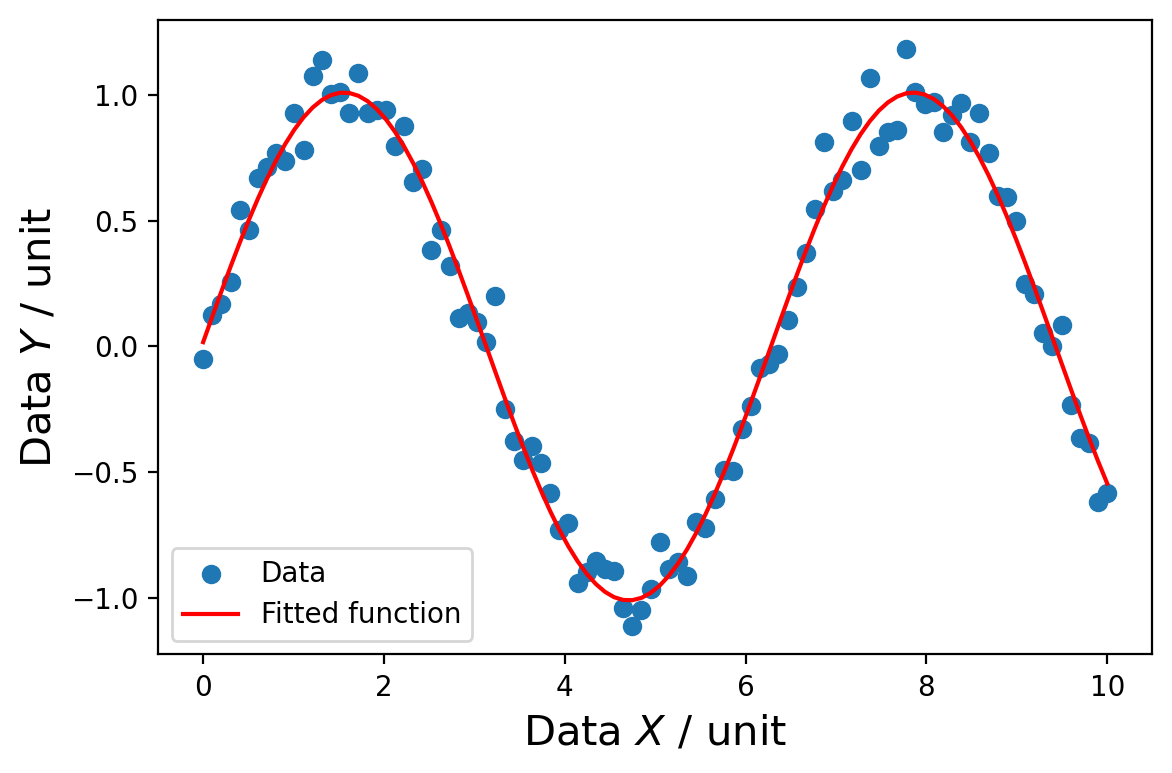
\includegraphics[scale=0.3]{figures/sin_fit_x_y.png}
    	\caption{Example plot that still needs a descriptive caption.}
        \label{fig:sin_fit_x_y}
    \end{figure}
\end{center}


\subsection{Comparing the fit to theoretical predictions} \label{sec:analysis_comparison}

\comment{A theoretical prediction could be made in the form of an equation, such as Eq.~\ref{eq:sine}:}
\begin{equation}
    y(x) = A \sin(\omega x + \phi) + \mu, \label{eq:sine}
\end{equation}
where $A$ is the amplitude of the sine wave, $\omega$ is the angular frequency, $\phi$ is the phase shift, and $\mu$ is the vertical offset or mean value around which the sine wave oscillates.

\comment{Because of the input function of \LaTeX, you can also save specific results as tex-text and import it later. For example the result of the amplitude was $A$ was $A = 1.011 \pm 0.014\,\mathrm{unit}$}

\subsection{A note on reproducibility (again)}\label{sec:analysis_reproducibility}

\comment{Until here, your manuscript is purely based on techniques. Note: Even random processes, like Monte Carlo sampling can be fixed for better reproducibility, but defining a \texttt{numpy.random.seed(PutIntegerValueHere)}. If you have done your job right, anyone should be able to take your code and run it on their computer to get the same results and plots as you (within machine precision). This also means: Write your code with useful comments, so that people can follow your steps.}

\SB{Do not forget to delete this subsection.}

\clearpage
%%%%%%%%%%%%%%%%%%%%%%%%%%%%%%%%%%%%%%%%%%%%%%%%%
%%%%%%%%%%%%%%%%%%%%%%%%%%%%%%%%%%%%%%%%%%%%%%%%%
\section{Discussion} \label{sec:discussion}

\comment{From here on, the exciting but debatable part of science begins: discussing what the results mean. Remember: People may dispute the conclusions that you draw from your analyses, so always back up statements with logical and analytical arguments or at least with quantities and uncertainties.}

\comment{Because we have identified (and likely iteratively refined) hypotheses in the introduction (Sec.~\ref{sec:hypotheses}), we can now easily return to them and discuss them in individual subsections:}

Having presented the analysis, we now put our results into the context of other work in terms of our initial aims: to analyze how ... (Section~\ref{sec:discussion_hypothesis1}), how much ...  (Section~\ref{sec:discussion_hypothesis2}), when (Section~\ref{sec:discussion_hypothesis3}), which (Section~\ref{sec:discussion_hypothesis4}), and where (Section~\ref{sec:discussion_hypothesis5}).

\comment{This may seem unreasonable now, but it will help your reader to navigate your discussion, once it has grown to several pages...}

\subsection{How ...?} \label{sec:discussion_hypothesis1}

\comment{Discussion of hypothesis 1: ...}

\subsection{How much ...?} \label{sec:discussion_hypothesis2}

\comment{Discussion of hypothesis 2: ...}

\subsection{When ...?} \label{sec:discussion_hypothesis3}

\comment{Discussion of hypothesis 3: ...}

\subsection{Which ...?} \label{sec:discussion_hypothesis4}

\comment{Discussion of hypothesis 4: ...}

\subsection{Where ...?} \label{sec:discussion_hypothesis5}

\comment{Discussion of hypothesis 5: ...}


\comment{This may not be the final format of your discussion, but I like to use it as a good and structured starting point. Ultimately, I always write down all of the hypotheses, analyses, the key results and figures from each analysis, and discussion in bullet points on my white board. That way I can easily make sure that I have a story line.}

\clearpage
%%%%%%%%%%%%%%%%%%%%%%%%%%%%%%%%%%%%%%%%%%%%%%%%%
%%%%%%%%%%%%%%%%%%%%%%%%%%%%%%%%%%%%%%%%%%%%%%%%%
\section{Conclusions} \label{sec:conclusions}

\comment{Because your analysis and discussion have stretched over multiple pages, and the abstract only allows you up to 250 words, this is the place where you can summarize the main results and conclusions that you have drawn, and put them into the context of the big picture problem that you wanted to contribute to.}

To conclude our study, we first iterate the main take-away of our research in Section~\ref{sec:conclusions_takeaway} before giving suggestions for future research in Section~\ref{sec:conclusions_future_research}.

\subsection{Take-away} \label{sec:conclusions_takeaway}

\comment{I like to write the take-away in bullet points and for each of them link back to sections and/or figures. For example:}

We have analyzed .... and find the following main results:
\begin{itemize}
    \item We have found a linear relationship between \textit{x} and \textit{y} (Section~\ref{sec:analysis_fitting} and Table~\ref{tab:sin_fit_x_y}).
    \item Our comparison of theoretical predictions with observations of  \textit{x} suggests ... (Fig.~\ref{fig:sin_fit_x_y}).
\end{itemize}

\subsection{Future research} \label{sec:conclusions_future_research}

\comment{What follow-up research should be done? What new questions arose from your research? Which investigations were beyond the scope of this paper?}

\comment{Finally, loop back to the big questions that your research and future research will contribute to by closing with a vision.}

\clearpage

%%%%%%%%%%%%%%%%%%%%%%%%%%%%%%%%%%%%%%%%%%%%%%%%%
%%%%%%%%%%%%%%%%%%%%%%%%%%%%%%%%%%%%%%%%%%%%%%%%%
\section*{Acknowledgments}

\comment{Acknowledge people(s) and support (if you got any). I would write for example:}

We acknowledge the traditional owners of the land on which the ANU stands, the Ngunnawal and Ngambri people. We pay our respects to elders past, and present and are proud to continue their tradition of surveying the night sky and its mysteries to better understand our Universe.

SB acknowledges support from the Australian Research Council under grant numbers DE240100150 and CE170100013.

%%%%%%%%%%%%%%%%%%%%%%%%%%%%%%%%%%%%%%%%%%%%%%%%%
%%%%%%%%%%%%%%%%%%%%%%%%%%%%%%%%%%%%%%%%%%%%%%%%%
\section*{Data Availability}

All code to reproduce the analysis and figures can be publicly accessed via \url{https://github.com/USERNAME/REPOSITORYNAME}.

%%%%%%%%%%%%%%%%%%%%%%%%%%%%%%%%%%%%%%%%%%%%%%%%%
%%%%%%%%%%%%%%%%%%%%%%%%%%%%%%%%%%%%%%%%%%%%%%%%%
\bibliographystyle{mnras}
\bibliography{bib}

%%%%%%%%%%%%%%%%%%%%%%%%%%%%%%%%%%%%%%%%%%%%%%%%%
%%%%%%%%%%%%%%%%%%%%%%%%%%%%%%%%%%%%%%%%%%%%%%%%%
%\begin{appendix}

%\section{Interesting information that is not vital for the main story of your paper}

%\end{appendix}

\end{document}